\usetikzlibrary{plotmarks}
\usepgfplotslibrary{groupplots}

\colorlet{linecolora}{blue}
\colorlet{linecolorb}{red}
\colorlet{linecolorc}{brown}
\colorlet{linecolord}{black}

\newcommand{\markOne}{*}
\newcommand{\markTwo}{triangle*}
\newcommand{\markThree}{square*}
\newcommand{\markFour}{diamond*}


\newcommand{\tikzPlotStylea}{

\begin{tikzpicture}
\draw[linecolora] plot[mark = \markOne] (0,0);
\end{tikzpicture}
}

\newcommand{\tikzPlotStyleb}{
\begin{tikzpicture}
\draw [linecolorb] plot[mark = \markTwo] (0,0);
\end{tikzpicture}
}

\newcommand{\tikzPlotStylec}{

\begin{tikzpicture}
\draw [linecolorc] plot[mark = \markThree] (0,0);
\end{tikzpicture}
}

\newcommand{\tikzPlotStyled}{

\begin{tikzpicture}
\draw [linecolord] plot[mark = \markFour] (0,0);
\end{tikzpicture}
}

\pgfplotsset{
plotoptsa/.style={only marks,color=linecolora,mark=\markOne},
plotoptsb/.style={only marks,color=linecolorb,mark=\markTwo},
plotoptsc/.style={only marks,color=linecolorc,mark=\markThree},
plotoptsd/.style={only marks,color=linecolord,mark=\markFour}
}


\newcommand{\addGroupPlotToFigure}[2]{
\addplot+[
		  plotoptsa,
          error bars/.cd,
		  y explicit, y dir=both,
		]
table[linecolora,x =x,y =y,y error =yp,col sep = comma]{../../data/#1-small-small-subplot-#2};
\addplot+[
		  plotoptsb,
          error bars/.cd,
		  y explicit, y dir=both,
		]
table[linecolorb,x =x,y =y,y error =yp,col sep = comma]{../../data/#1-small-big-subplot-#2};
\addplot+[
		  plotoptsc,
          error bars/.cd,
		  y explicit, y dir=both,
		]
table[linecolorc,x =x,y =y,y error =yp,col sep = comma]{../../data/#1-big-small-subplot-#2};
\addplot+[
 		  plotoptsd,
          error bars/.cd,
		  y explicit, y dir=both,
		]
table[linecolord,x =x,y =y,y error =yp,col sep = comma]{../../data/#1-big-big-subplot-#2};
}

\newcommand{\addGhostGroupPlotToFigure}[2]{
\addplot+[
		  draw = none,
		]
table[draw = none,mark =none, x =x,y expr = {\thisrow{y}+\thisrow{yp}},col sep = comma]{../../data/#1-small-small-subplot-#2};
\addplot+[
          draw = none,
		]
table[draw = none,mark =none, x =x,y expr = {\thisrow{y}+\thisrow{yp}},col sep = comma]{../../data/#1-small-big-subplot-#2};
\addplot+[
          draw = none,
		]
table[draw = none,mark =none, x =x,y expr = {\thisrow{y}+\thisrow{yp}},col sep = comma]{../../data/#1-big-small-subplot-#2};
\addplot+[
          draw = none,
		]
table[draw = none,mark =none, x =x,y expr = {\thisrow{y}+\thisrow{yp}},col sep = comma]{../../data/#1-big-big-subplot-#2};
\addplot+[
		  draw = none,
		]
table[draw = none,mark =none, x =x,y expr = {\thisrow{y}-\thisrow{ym}},col sep = comma]{../../data/#1-small-small-subplot-#2};
\addplot+[
          draw = none,
		]
table[draw = none,mark =none, x =x,y expr = {\thisrow{y}-\thisrow{ym}},col sep = comma]{../../data/#1-small-big-subplot-#2};
\addplot+[
          draw = none,
		]
table[draw = none,mark =none, x =x,y expr = {\thisrow{y}-\thisrow{ym}},col sep = comma]{../../data/#1-big-small-subplot-#2};
\addplot+[
          draw = none,
		]
table[draw = none, mark =none, x =x,y expr = {\thisrow{y}-\thisrow{ym}},col sep = comma]{../../data/#1-big-big-subplot-#2};
}
\newcommand{\makeFigureAllSizes}[2]{
\pgfplotssetlayers
\begin{tikzpicture}
\begin{groupplot}[group style = {group size =2 by 2,
			group name = the plots,
			xlabels at = edge bottom,
			ylabels at = edge left
                                },
			width = .4\linewidth,
			height = .3\linewidth,
			scale only axis = true,		    
   			xlabel = {Fraction Consumers as parasites},
			ylabel = {#2},
			x label style = {font=\tiny},
			y label style = {font=\tiny},
		    legend style={ ,at={(-.15,-.23)},
						   anchor=north,
						   font=\tiny},
			legend columns = 4,
			grid = both,
			unbounded coords = jump,
			%ymin = 0,ymax = 1,
]
\nextgroupplot[xticklabels={}]
\addGroupPlotToFigure{#1}{1}
\addGhostGroupPlotToFigure{#1}{2}
\addGhostGroupPlotToFigure{#1}{3}
\addGhostGroupPlotToFigure{#1}{4}
\nextgroupplot[xticklabels={},yticklabels={}]
\addGroupPlotToFigure{#1}{2}
\addGhostGroupPlotToFigure{#1}{1}
\addGhostGroupPlotToFigure{#1}{3}
\addGhostGroupPlotToFigure{#1}{4}
\nextgroupplot
\addGroupPlotToFigure{#1}{3}
\addGhostGroupPlotToFigure{#1}{2}
\addGhostGroupPlotToFigure{#1}{1}
\addGhostGroupPlotToFigure{#1}{4}
\nextgroupplot[yticklabels={}]
\addGroupPlotToFigure{#1}{4}
\addGhostGroupPlotToFigure{#1}{2}
\addGhostGroupPlotToFigure{#1}{3}
\addGhostGroupPlotToFigure{#1}{1}
\legend{$Z_f=10;Z_p = 10^{-3}$,
$Z_f=10;Z_p = 10^{-4}$,
$Z_f=100;Z_p = 10^{-3}$,
$Z_f=100;Z_p = 10^{-4}$}
\end{groupplot}
\node [text width =.5\linewidth,align=center,anchor=south] at (the plots c1r1.north) {\subcaption[]{ Null model\label{fig:#1-a}}};
\node [text width =.5\linewidth,align=center,anchor=south] at (the plots c2r1.north) {\subcaption[]{Refuge\label{fig:#1-b}}};
\node [text width =.5\linewidth,align=center,anchor=south] at (the plots c1r2.north) {\subcaption[]{Concomittant \label{fig:#1-c}}};
\node [text width =.5\linewidth,align=center,anchor=south] at (the plots c2r2.north) {\subcaption[]{Refuge with Concomittant\label{fig:#1-d}}};
\begin{pgfonlayer}{axis background}
\node [opacity = 0.4,] at (the plots c1r1.center) {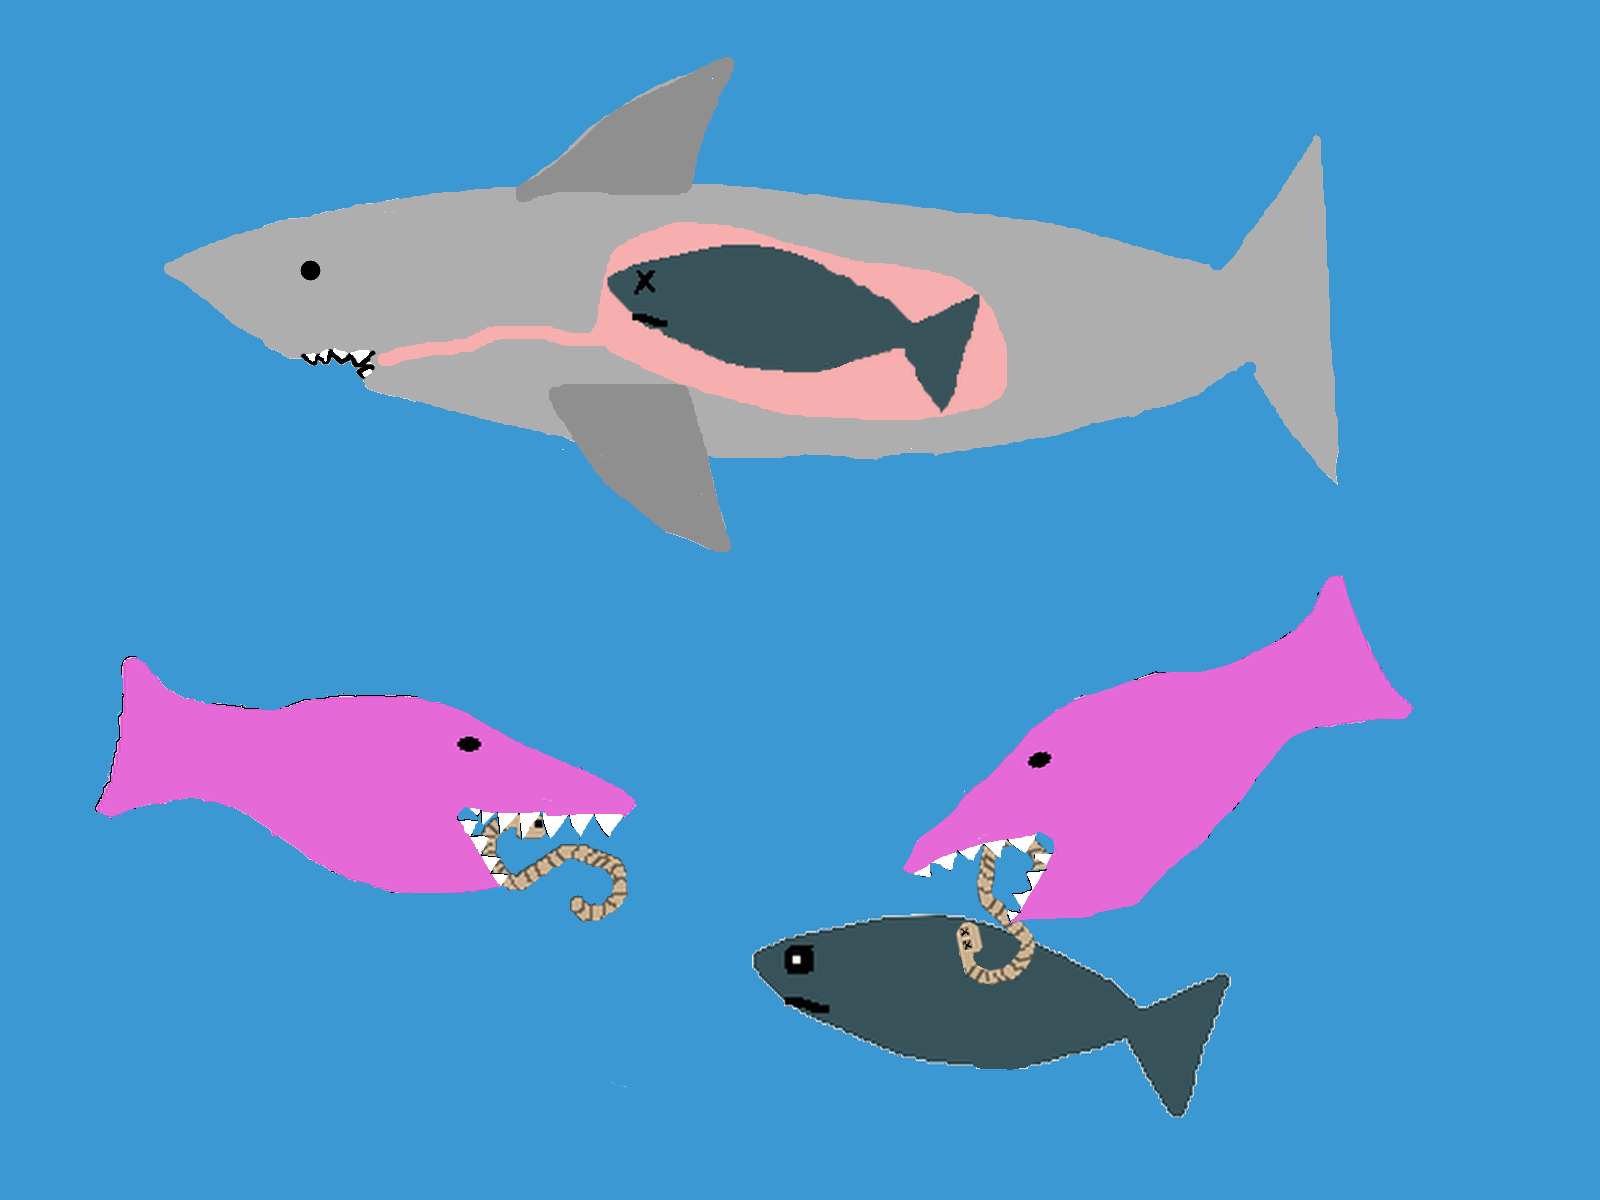
\includegraphics[width=.4\linewidth]{../../figures/Null.png}};
\node [opacity = 0.4,] at (the plots c2r1.center) {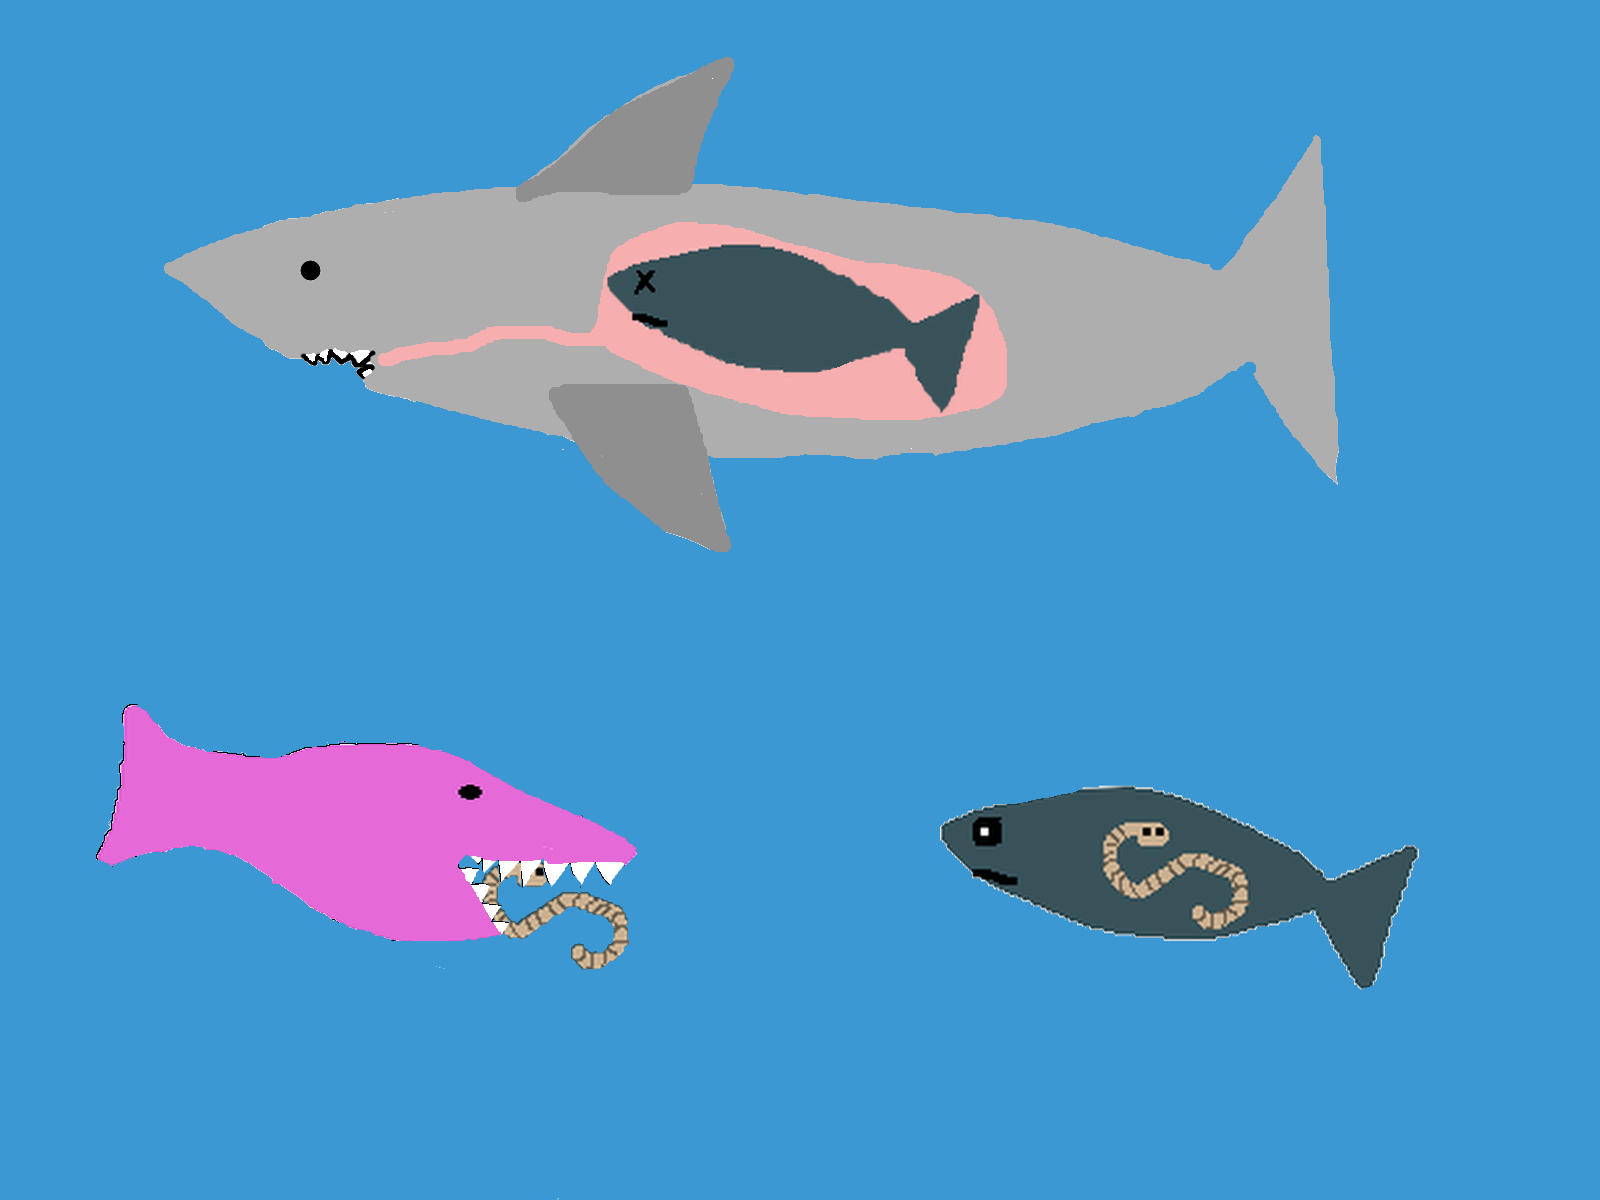
\includegraphics[width=.4\linewidth]{../../figures/Null+Ref.png}};
\node [opacity = 0.4,] at (the plots c1r2.center) {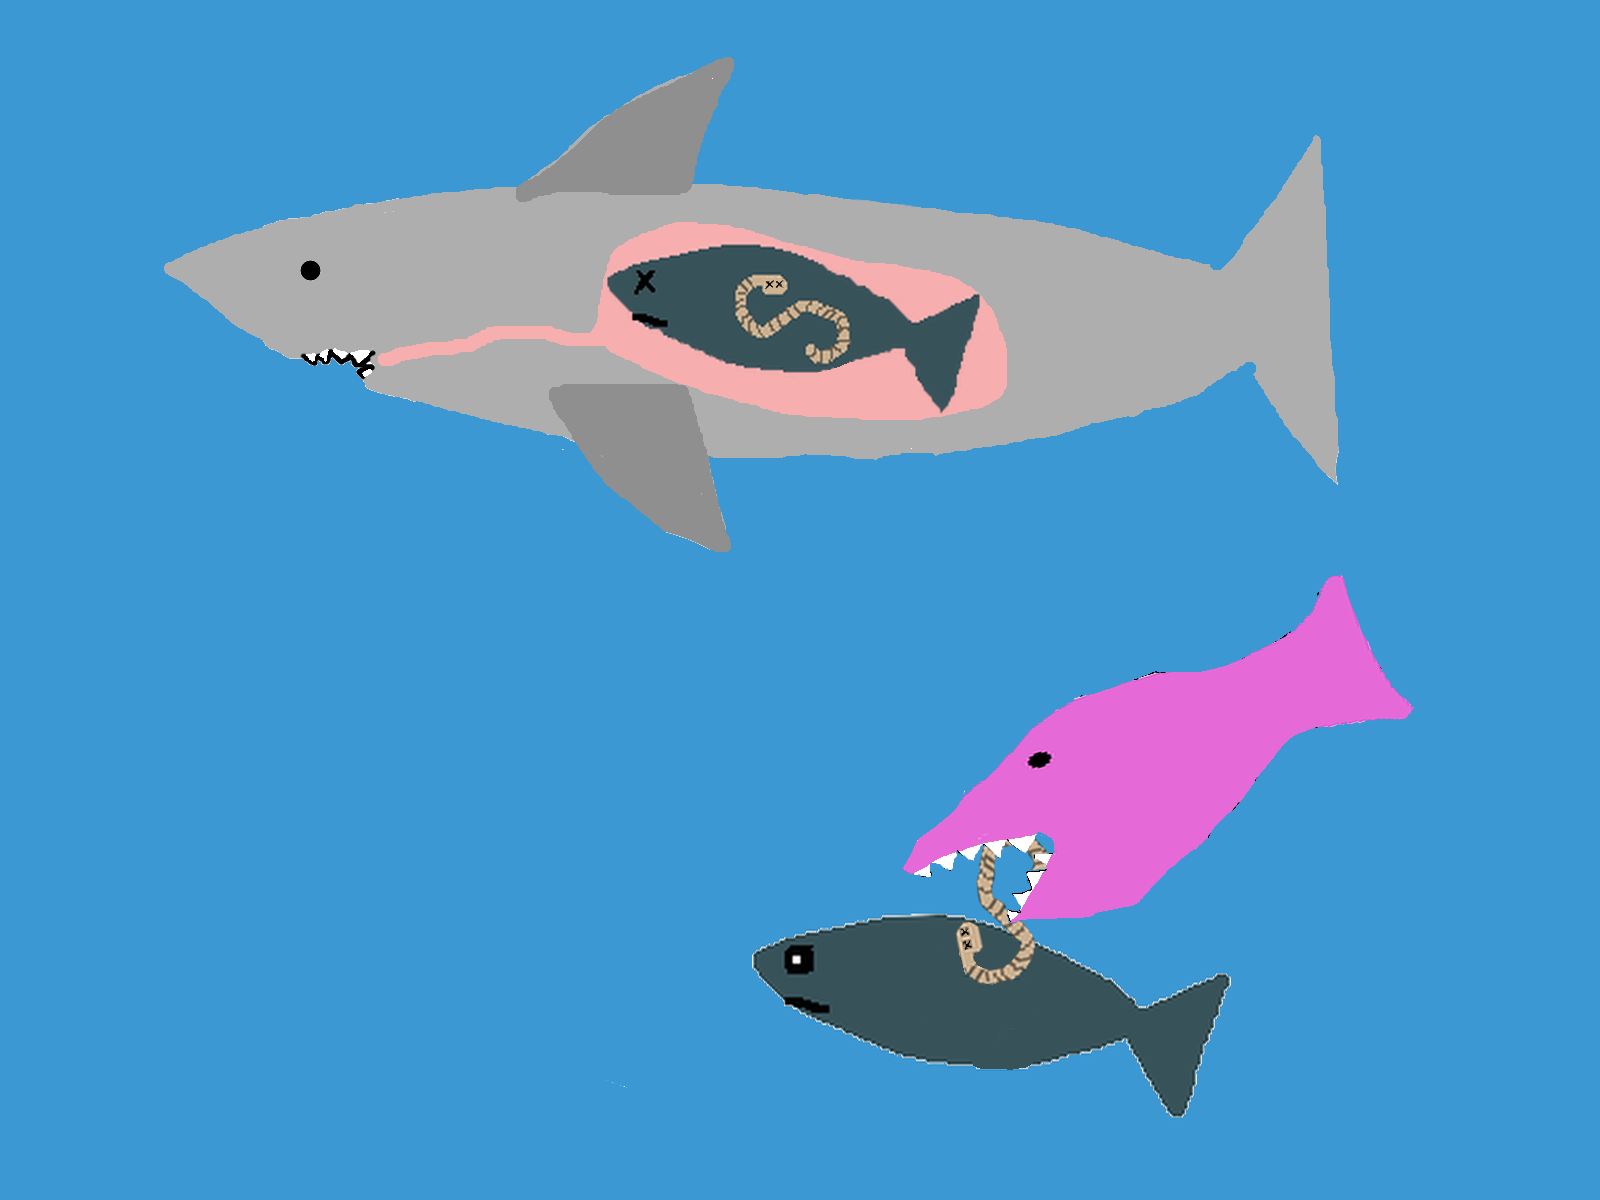
\includegraphics[width=.4\linewidth]{../../figures/Null+Con.png}};
\node [opacity = 0.4,] at (the plots c2r2.center) {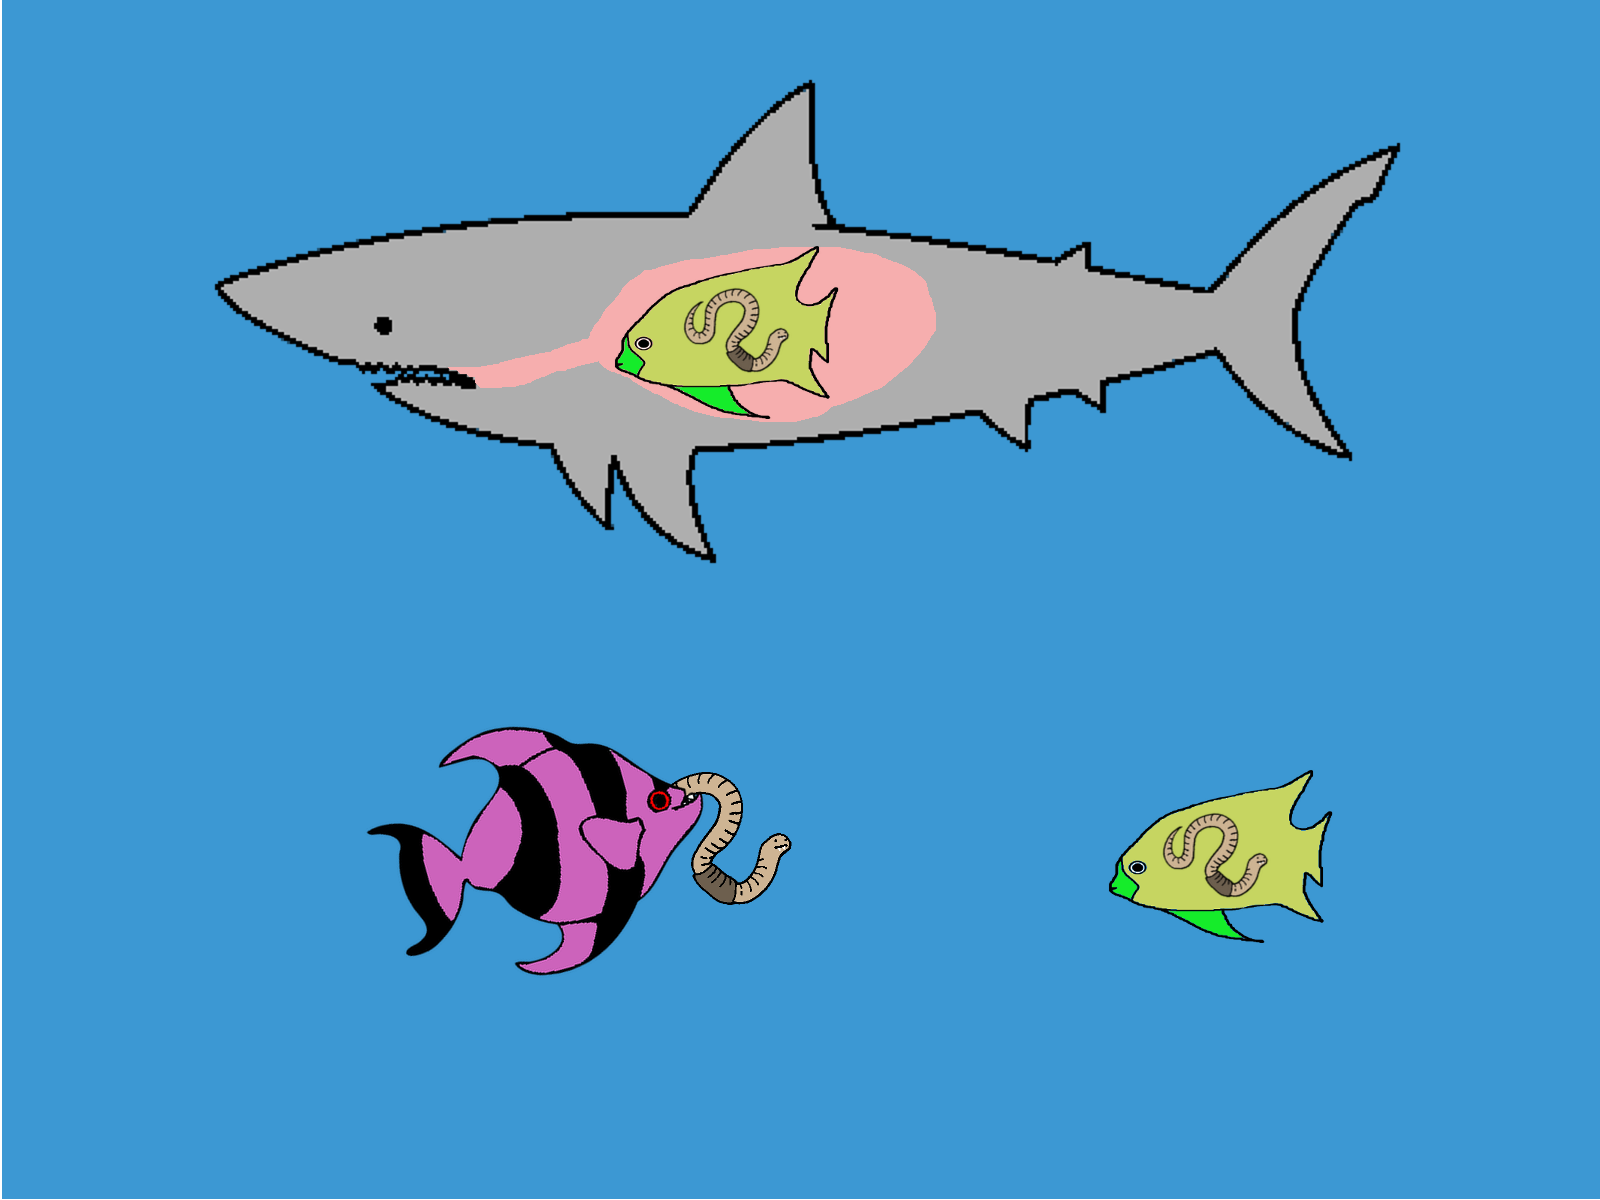
\includegraphics[width=.4\linewidth]{../../figures/Con+Ref.png}};
\end{pgfonlayer}
\end{tikzpicture}
}

\newcommand{\makeFigureTwoModels}[2]{
\pgfplotstableread{../../data/#1-small-small-subplot-1}\tableA
\pgfplotstableread{../../data/#1-small-small-subplot-4}\tableD
\pgfplotssetlayers
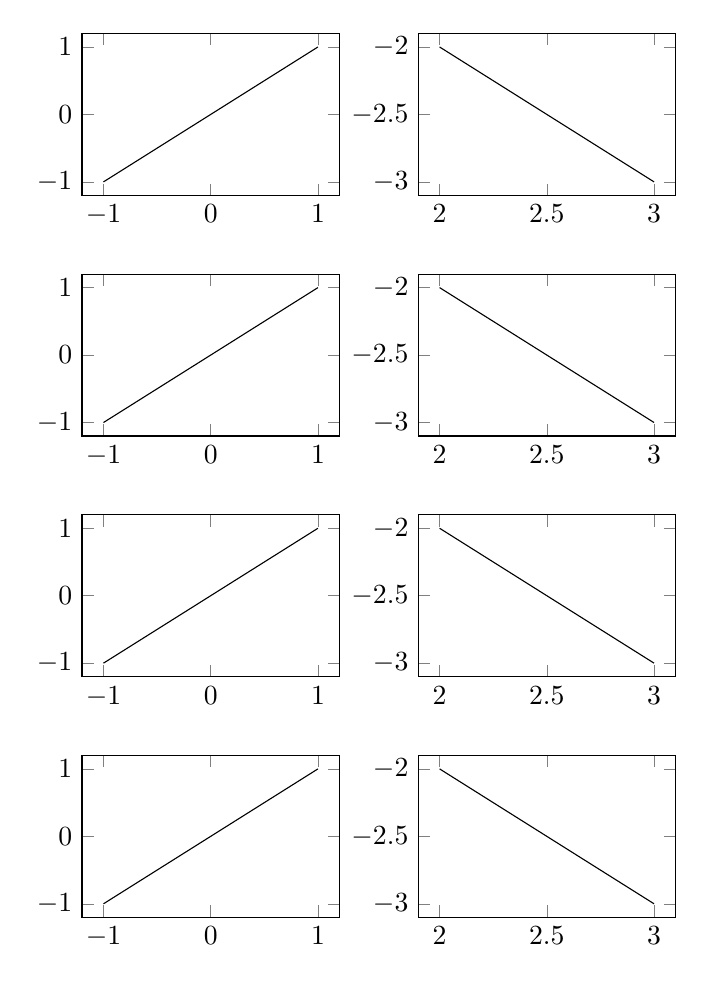
\begin{tikzpicture}
\begin{groupplot}[group style = {group size = 2 by 4,
			%group name = the plots,
			%xlabels at = edge bottom,
			%ylabels at = edge left,
                                },
			width = .4\linewidth,
			height = .3\linewidth,
			%scale only axis = true,		    
   			%xlabel = {Fraction Consumers as parasites},
			%ylabel = {#2},
			%x label style = {font=\tiny},
			%y label style = {font=\tiny},
		        %legend style={at={(-.15,-.23)},
		        %      	      anchor=north,
		       % 	      font=\tiny},
		%	legend columns = 4,
		%	grid = both,
		%	unbounded coords = jump,
			%ymin = 0,ymax = 1,
]
\nextgroupplot
\addplot[domain=-1:1] {x};
%\addGroupPlotToFigure{#1}{1};
%\addGhostGroupPlotToFigure{#1}{4};
\nextgroupplot
\addplot[domain = 2:3] {-x};
\nextgroupplot
\addplot[domain=-1:1] {x};
\nextgroupplot
\addplot[domain = 2:3] {-x};
\nextgroupplot
\addplot[domain=-1:1] {x};
\nextgroupplot
\addplot[domain = 2:3] {-x};
\nextgroupplot
\addplot[domain=-1:1] {x};
\nextgroupplot
\addplot[domain = 2:3] {-x};
%\addGroupPlotToFigure{#1}{4};
%\addGhostGroupPlotToFigure{#1}{1};
%\legend{$Z_f=10;Z_p = 10^{-3}$,
%$Z_f=10;Z_p = 10^{-4}$,
%$Z_f=100;Z_p = 10^{-3}$,
%$Z_f=100;Z_p = 10^{-4}$}
\end{groupplot}
%\node [text width =.5\linewidth,align=center,anchor=south] at (the plots c1r1.north) {\subcaption[]{ Null Model\label{fig:#1-a}}};
%\node [text width =.5\linewidth,align=center,anchor=south] at (the plots c2r1.north) {\subcaption[]{Parasite Model\label{fig:#1-b}}};
%\begin{pgfonlayer}{axis background}
%\node [opacity = 0.4,] at (the plots c1r1.center) {\includegraphics[width=.4\linewidth]{../../figures/Null.png}};
%\node [opacity = 0.4,] at (the plots c2r1.center) {\includegraphics[width=.4\linewidth]{../../figures/Con+Ref.png}};
%\end{pgfonlayer}
\end{tikzpicture}
}

\newcommand{\makeFigureAllModels}[2]{
\begin{tikzpicture}
\begin{axis}[
		    xlabel = {Fraction Consumers as parasites},
			ylabel = {#2},
		    legend style={ ,at={(-.45,-.33)},
						   ,anchor=south},
			legend columns = 2,
]

\addplot+[
		  only marks, mark = o,
          error bars/.cd,
		  y explicit, y dir=both,
		]
table[blue, x =x,y =y,y error =yp,col sep = comma]{../../data/#1-1};
\addplot+[
		  only marks, mark = triangle,
          error bars/.cd,
		  y explicit, y dir=both,
		]
table[red,x =x,y =y,y error =yp,col sep = comma]{../../data/#1-2};
\addplot+[
		  only marks, mark = square,
          error bars/.cd,
		  y explicit, y dir=both,
		]
table[brown,x =x,y =y,y error =yp,col sep = comma]{../../data/#1-3};
\addplot+[
		  only marks, mark = diamond,
          error bars/.cd,
		  y explicit, y dir=both,
		]
table[black,x =x,y =y,y error =yp,col sep = comma]{../../data/#1-4};
\legend{Null Model,
 Host Refuge,
 Concomittant Only,
 Refuge with Concomittant}
\end{axis}
\end{tikzpicture}
}


\newcommand{\addMainEffectPlotToFigureToFigure}[2]{
\addplot+[
		  plotoptsa,
          error bars/.cd,
		  y explicit, y dir=both,
		]
table[linecolora,x =x,y =y,y error =yp,col sep = comma]{../../data/#1-effect-on-subplot-#2};
\addplot+[
		  plotoptsb,
          error bars/.cd,
		  y explicit, y dir=both,
		]
table[linecolorb,x =x,y =y,y error =yp,col sep = comma]{../../data/#1-effect-off-subplot-#2};
}

\newcommand{\addMainEffectGhostGroupPlotToFigure}[2]{
\addplot+[
		  draw = none,
		]
table[draw = none,mark =none, x =x,y expr = {\thisrow{y}+\thisrow{yp}},col sep = comma]{../../data/#1-effect-on-subplot-#2};
\addplot+[
          draw = none,
		]
table[draw = none,mark =none, x =x,y expr = {\thisrow{y}+\thisrow{yp}},col sep = comma]{../../data/#1-effect-off-subplot-#2};
\addplot+[
		  draw = none,
		]
table[draw = none,mark =none, x =x,y expr = {\thisrow{y}-\thisrow{ym}},col sep = comma]{../../data/#1-effect-on-subplot-#2};
\addplot+[
          draw = none,
		]
table[draw = none,mark =none, x =x,y expr = {\thisrow{y}-\thisrow{ym}},col sep = comma]{../../data/#1-effect-off-subplot-#2};
}
\newcommand{\makeMainEffectsFigure}[2]{
\pgfplotssetlayers
\begin{tikzpicture}
\begin{groupplot}[group style = {group size =2 by 2,
			group name = the plots,
			xlabels at = edge bottom,
			ylabels at = edge left
                                },
			width = .4\linewidth,
			height = .3\linewidth,
			scale only axis = true,		    
   			xlabel = {Fraction Consumers as parasites},
			ylabel = {#2},
			x label style = {font=\tiny},
			y label style = {font=\tiny},
		    legend style={ ,at={(-.15,-.23)},
						   anchor=north,
						   font=\tiny},
			legend columns = 4,
			grid = both,
			unbounded coords = jump,
			%ymin = 0,ymax = 1,
]
\nextgroupplot[xticklabels={}]
\addMainEffectPlotToFigureToFigure{#1}{1}
\addMainEffectGhostGroupPlotToFigure{#1}{2}
\addMainEffectGhostGroupPlotToFigure{#1}{3}
\addMainEffectGhostGroupPlotToFigure{#1}{4}
\nextgroupplot[xticklabels={},yticklabels={}]
\addMainEffectGhostGroupPlotToFigure{#1}{1}
\addMainEffectPlotToFigureToFigure{#1}{2}
\addMainEffectGhostGroupPlotToFigure{#1}{3}
\addMainEffectGhostGroupPlotToFigure{#1}{4}
\nextgroupplot
\addMainEffectGhostGroupPlotToFigure{#1}{1}
\addMainEffectGhostGroupPlotToFigure{#1}{2}
\addMainEffectPlotToFigureToFigure{#1}{3}
\addMainEffectGhostGroupPlotToFigure{#1}{4}
\nextgroupplot[yticklabels={}]
\addMainEffectGhostGroupPlotToFigure{#1}{1}
\addMainEffectGhostGroupPlotToFigure{#1}{2}
\addMainEffectGhostGroupPlotToFigure{#1}{3}
\addMainEffectPlotToFigureToFigure{#1}{4}
\legend{$Z_f=10;Z_p = 10^{-3}$,
$Z_f=10;Z_p = 10^{-4}$,
$Z_f=100;Z_p = 10^{-3}$,
$Z_f=100;Z_p = 10^{-4}$}
\end{groupplot}
\node [text width =.5\linewidth,align=center,anchor=south] at (the plots c1r1.north) {\subcaption[]{ Null model\label{fig:#1-a}}};
\node [text width =.5\linewidth,align=center,anchor=south] at (the plots c2r1.north) {\subcaption[]{Refuge\label{fig:#1-b}}};
\node [text width =.5\linewidth,align=center,anchor=south] at (the plots c1r2.north) {\subcaption[]{Concomittant \label{fig:#1-c}}};
\node [text width =.5\linewidth,align=center,anchor=south] at (the plots c2r2.north) {\subcaption[]{Refuge with Concomittant\label{fig:#1-d}}};
\begin{pgfonlayer}{axis background}
\node [opacity = 0.4,] at (the plots c1r1.center) {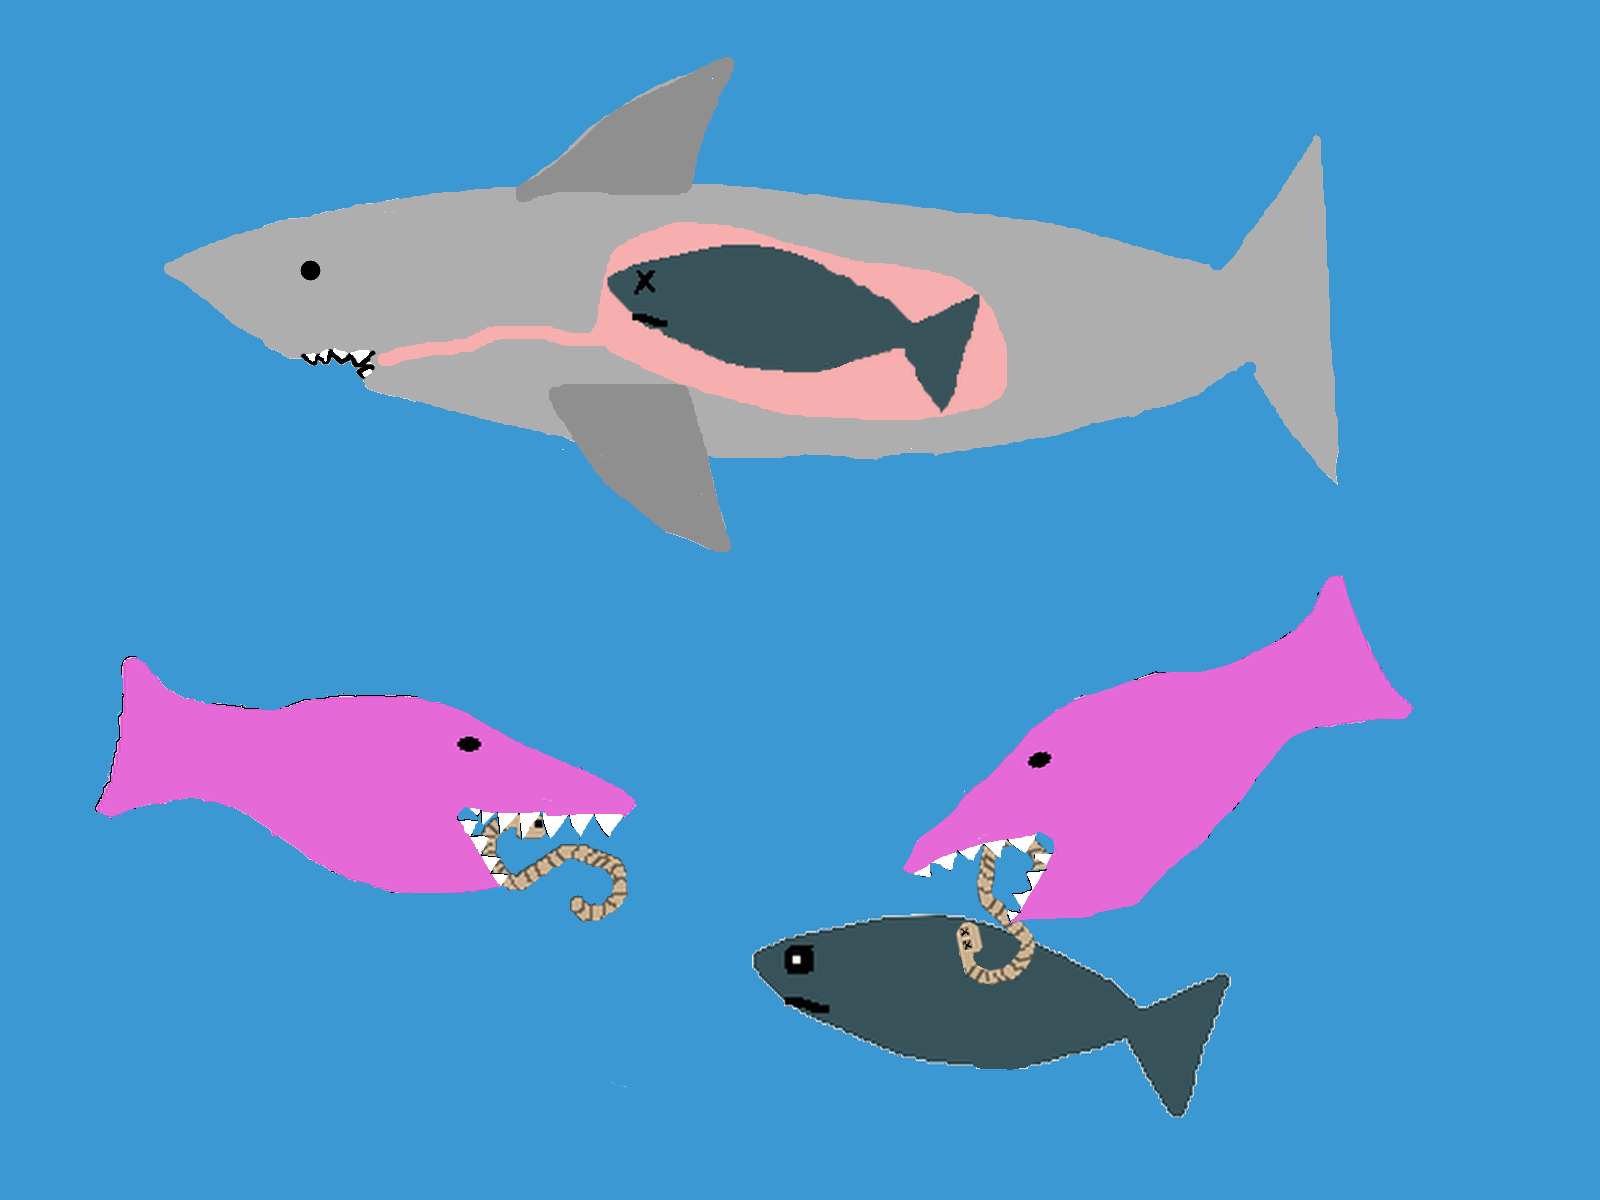
\includegraphics[width=.4\linewidth]{../../figures/Null.png}};
\node [opacity = 0.4,] at (the plots c2r1.center) {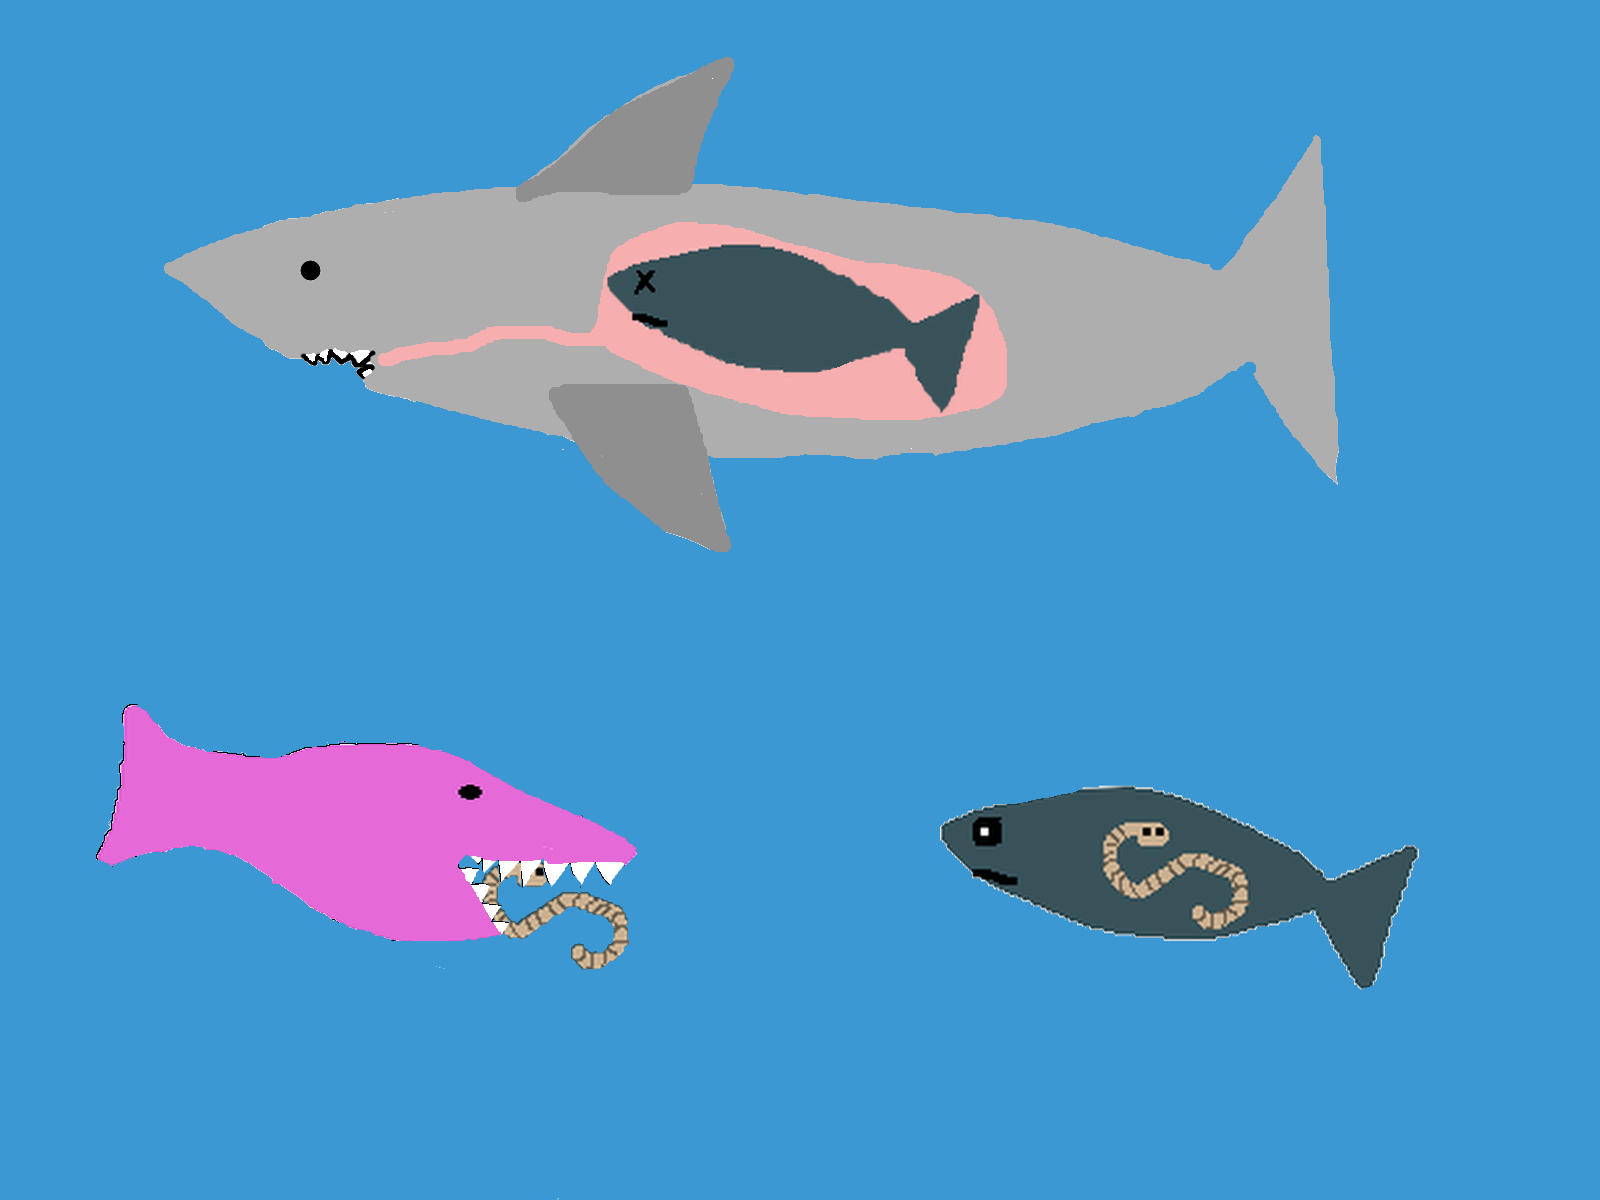
\includegraphics[width=.4\linewidth]{../../figures/Null+Ref.png}};
\node [opacity = 0.4,] at (the plots c1r2.center) {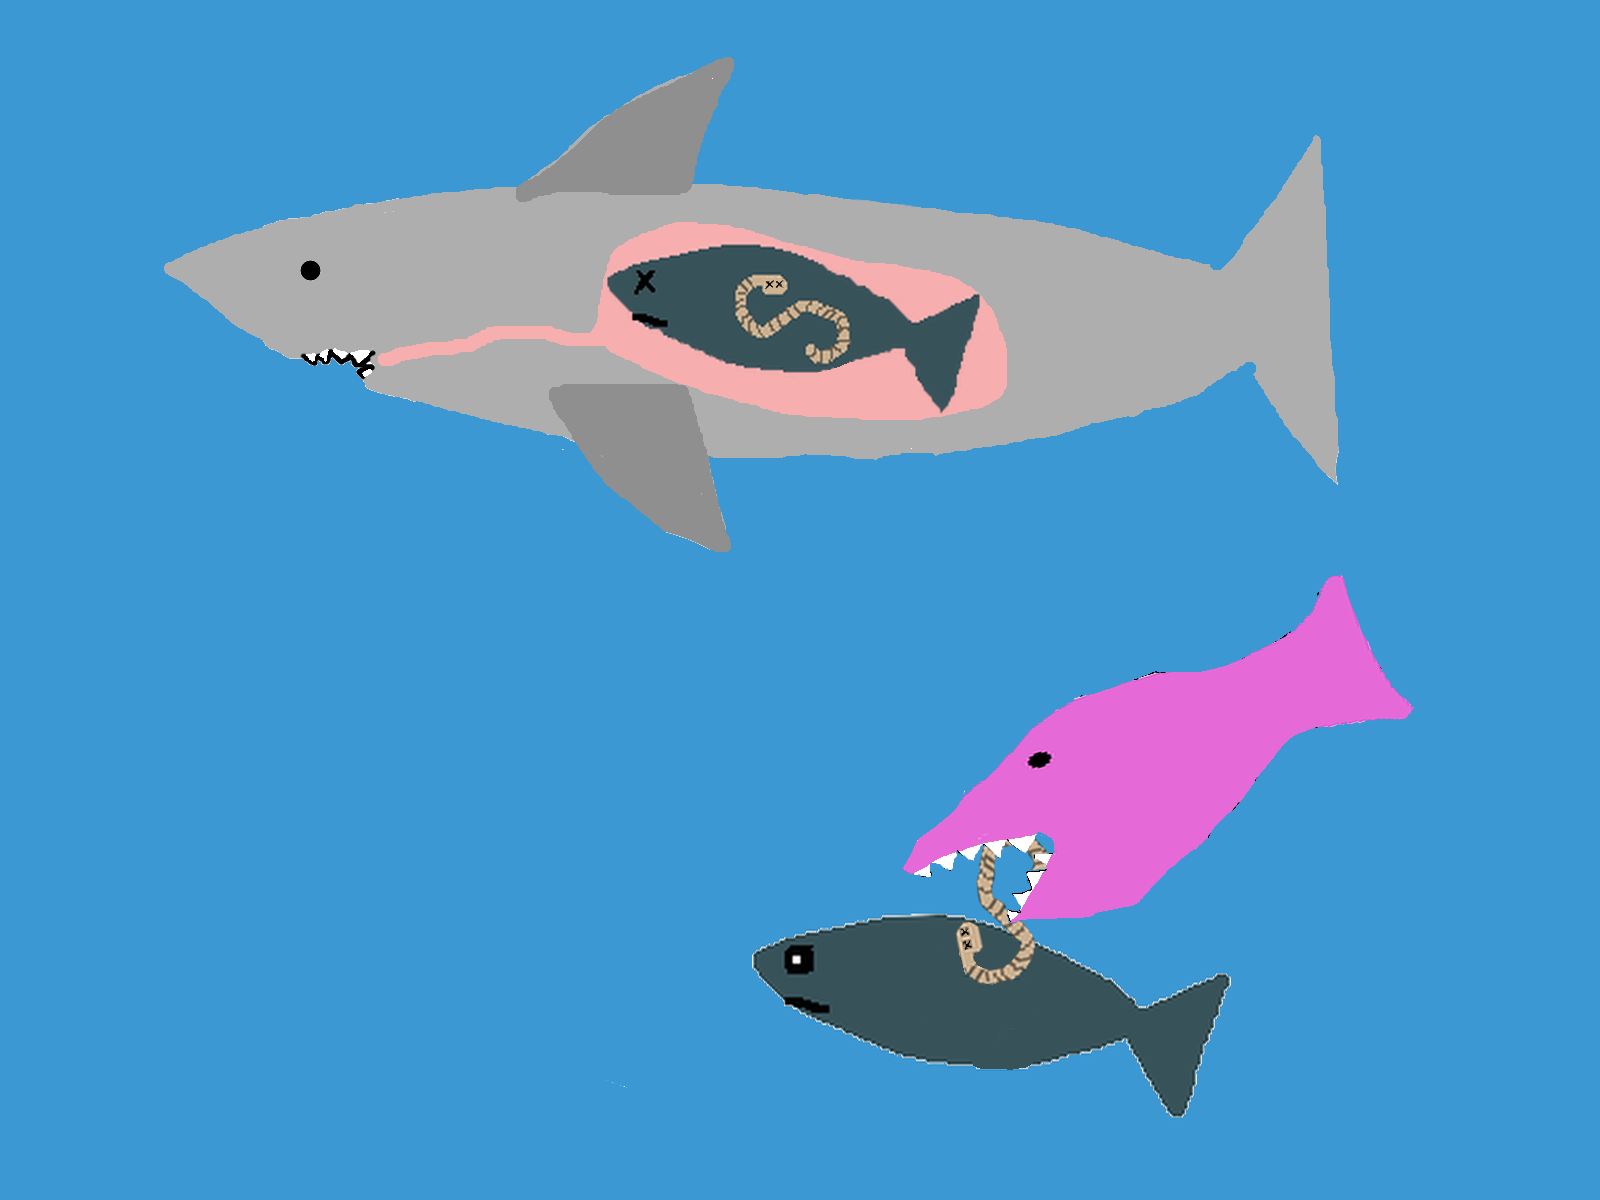
\includegraphics[width=.4\linewidth]{../../figures/Null+Con.png}};
\node [opacity = 0.4,] at (the plots c2r2.center) {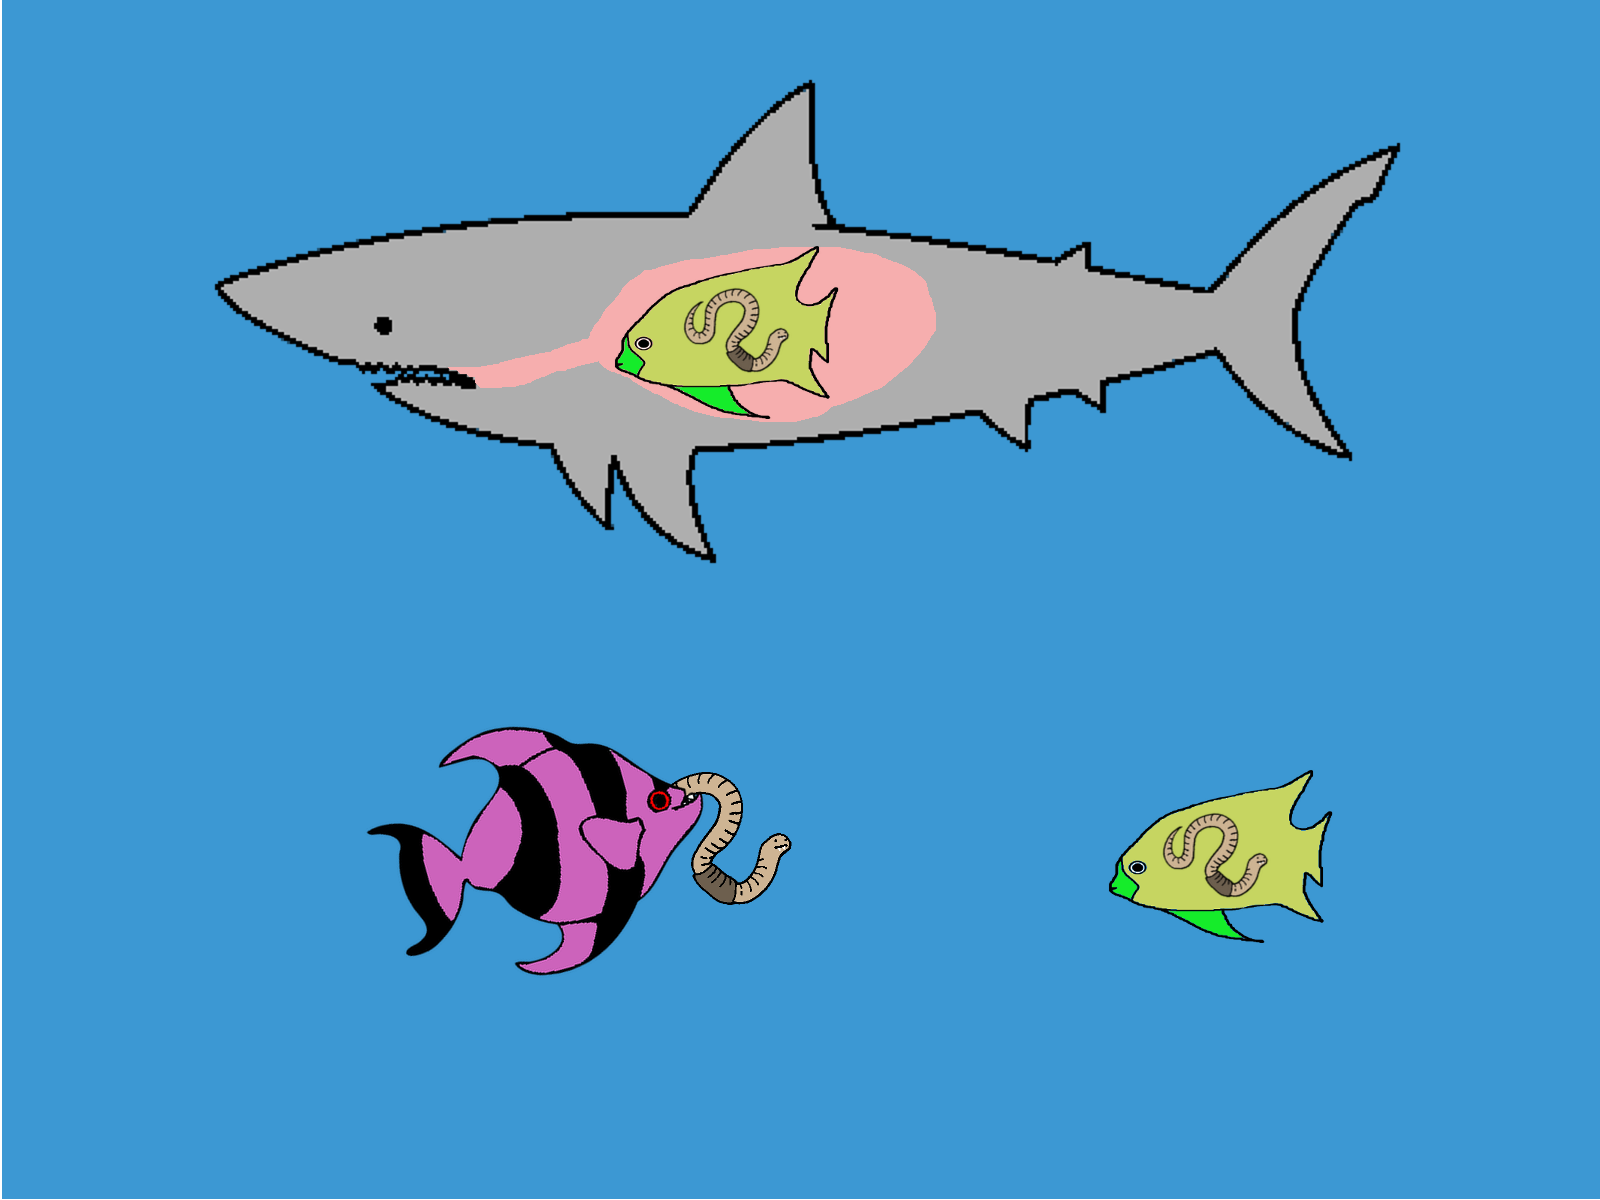
\includegraphics[width=.4\linewidth]{../../figures/Con+Ref.png}};
\end{pgfonlayer}
\end{tikzpicture}
}
